\section{电热器}\label{sec:9-5}

电流的热效应有着广泛的应用。电热器就是利用电流的热效应制成的加热设备。
电烙铁、电炉、电熨斗(图 \ref{fig:9-6}) 都是常见的电热器。

\begin{figure}[htbp]
    \centering
    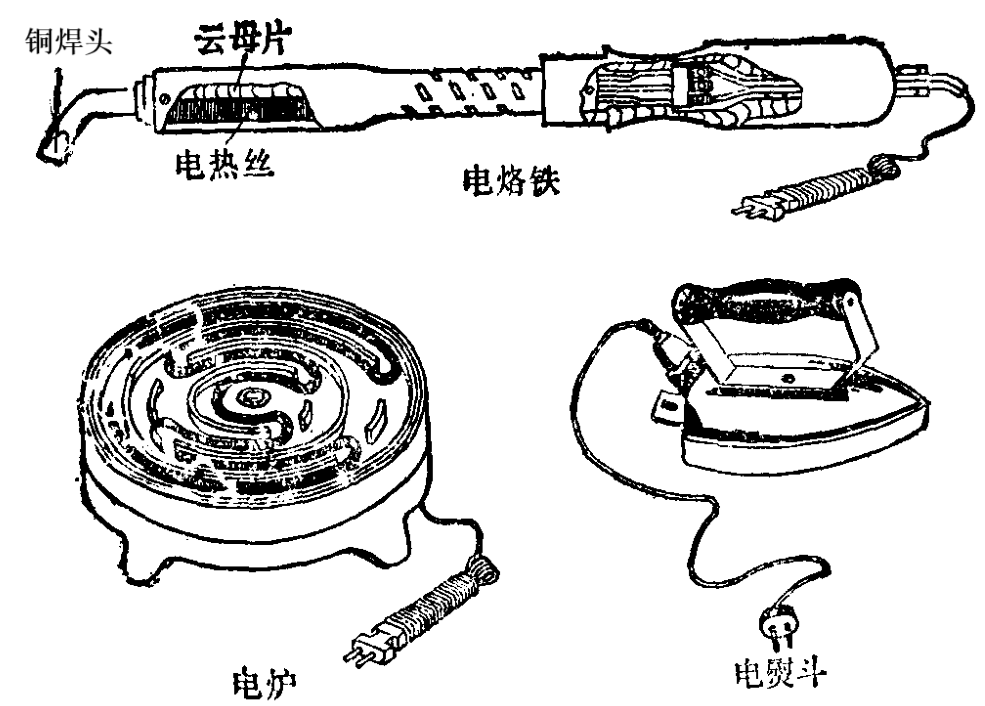
\includegraphics[width=0.8\textwidth]{../pic/czwl2-ch9-6}
    \caption{}\label{fig:9-6}
\end{figure}

电热器的主要组成部分是发热体。
发热体是由电阻率大、熔点高的合金丝绕在绝缘材料上做成的。
图 \ref{fig:9-6} 的上图表示出了电烙铁的内部构造。

烘干物品的电烘箱,爆破时引发炸药的电热装置,高空飞行员穿的衣服里的电热保温装置,等等,也都是电热器。
它们的构造和用途虽然不同,但原理都一样。

利用电流热效应和物体热膨胀现象,可以制成自动保持温度恒定的电热器——恒温箱。

\begin{figure}[htbp]
    \centering
    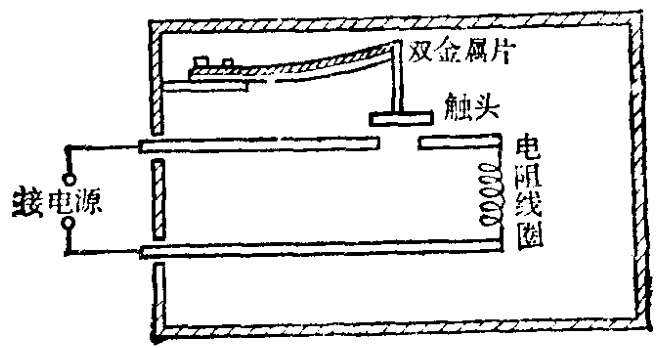
\includegraphics[width=0.4\textwidth]{../pic/czwl2-ch9-7}
    \caption{}\label{fig:9-7}
\end{figure}

图 \ref{fig:9-7} 是一种恒温箱的示意图。
当恒温箱内的温度超过规定数值时,双金属片向上弯曲,触头分开,电路切断,电阻线圈不发热,恒温箱内温度下降。
当温度低于规定的数值时,双金属片向下弯曲,触头闭合,电路接通,电阻线圈发热。
这样就使恒温箱内的温度保持恒定。

恒温箱是工农业生产和科学研究中的一种常用设备。
养禽业中使用的电热孵卵器就是一个大的恒温箱,能把箱内温度保持在 37.8 ℃ 左右,上下不超过 0.5 ℃。


\lianxi

(1) 将长度和横截面积完全相等的镍铬合金丝和铁丝照图 \ref{fig:9-8} 甲那样串联在电路中,
在镍铬合金丝和铁丝下面用蜡(或凡士林)粘上几根火柴,当接通电源后,哪些火柴先掉下来?为什么?
如果照图 \ref{fig:9-8} 乙那样并联在电路中,当接通电源后,哪些火柴先掉下来?为什么?有条件的同学可以做一做。

\begin{figure}[htbp]
    \centering
    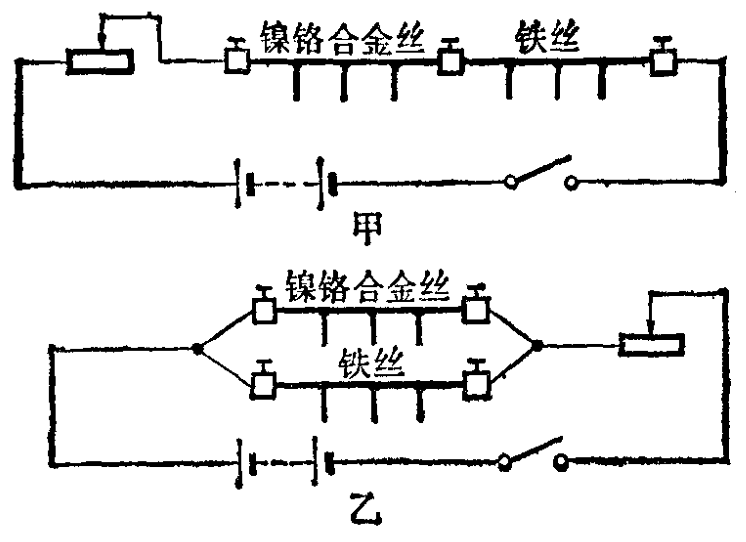
\includegraphics[width=0.7\textwidth]{../pic/czwl2-ch9-8}
    \caption{}\label{fig:9-8}
\end{figure}

(2) 电炉丝热得发红,而跟电炉丝连接着的铜导线却不怎么热,为什么?

(3) 某导体的电阻是 2 欧姆,当 1 安培的电流通过时,1 分钟产生多少焦耳的热量?

(4) 一只 “220V \; 45W” 的电烙铁,在额定电压下使用,每分钟产生的热量是多少?

(5) 某课外小组的同学自制了一只电烙铁。这只电烙铁正常工作的电阻是 1210 欧姆,
它的额定电压是 220 伏特,它的电功率是多大? 通电 10 分钟产生多少热量?

(6) 某校师生为了开展科学实验,自制了一台电烘箱,当它的电阻丝通过的电流是 5 安培时,
每分钟可产生 $6.6 \times 10^4$ 焦耳的热量。求这台电烘箱的电功率及电阻丝工作时的电阻。

